\let\negmedspace\undefined
\let\negthickspace\undefined
\documentclass[journal]{IEEEtran}
\usepackage[a5paper, margin=10mm, onecolumn]{geometry}
%\usepackage{lmodern} % Ensure lmodern is loaded for pdflatex
\usepackage{tfrupee} % Include tfrupee package

\setlength{\headheight}{1cm} % Set the height of the header box
\setlength{\headsep}{0mm}     % Set the distance between the header box and the top of the text

\usepackage{gvv-book}
\usepackage{gvv}
\usepackage{cite}
\usepackage{amsmath,amssymb,amsfonts,amsthm}
\usepackage{algorithmic}
\usepackage{graphicx}
\usepackage{textcomp}
\usepackage{xcolor}
\usepackage{txfonts}
\usepackage{listings}
\usepackage{enumitem}
\usepackage{mathtools}
\usepackage{gensymb}
\usepackage{comment}
\usepackage[breaklinks=true]{hyperref}
\usepackage{tkz-euclide} 
\usepackage{listings}
% \usepackage{gvv}                                        
\def\inputGnumericTable{}                                 
\usepackage[latin1]{inputenc}                                
\usepackage{color}                                            
\usepackage{array}                                            
\usepackage{longtable}                                       
\usepackage{calc}                                             
\usepackage{multirow}                                         
\usepackage{hhline}                                           
\usepackage{ifthen}                                           
\usepackage{lscape}
\begin{document}

\bibliographystyle{IEEEtran}
\vspace{3cm}

\title{12.8.3.1.2}
\author{EE24BTECH11019 - Dwarak A}
% \maketitle
% \newpage
% \bigskip
{\let\newpage\relax\maketitle}

\renewcommand{\thefigure}{\theenumi}
\renewcommand{\thetable}{\theenumi}
\setlength{\intextsep}{10pt} % Space between text and floats


\numberwithin{equation}{enumi}
\numberwithin{figure}{enumi}
\renewcommand{\thetable}{\theenumi}

\textbf{Question:}

Find the area under the given curves and given lines:
\begin{align}
    y &= x^4 \\
    x &= 1 \\
    x &= 5 \\
    y &= 0 \text{\quad(x-axis)}
\end{align}

\solution

\medskip

\textbf{Theoretical Solution:}

Area between lines and curve $A$,
\begin{align}
    A &= \int\limits_{1}^{5}x^4dx \\
    &= \frac{x^5}{5}\Big|_{x=5} - \frac{x^5}{5}\Big|_{x=1} \\
    &= \frac{3125}{5} - \frac{1}{5} \\
    &= 624.8
\end{align}

\medskip

\textbf{Simulated Solution (Trapezoidal Rule):}

Taking trapezoid shaped strips of small area and adding them all up. Say we have to find the area of $y\brak{x}$ from $x=x_0$ to $x=x_n$, discretize points on the $x$ axis $x_0, x_1, x_2, \dots, x_n$ such that they are equally spaced with step-size $h$. \newline
Sum of all trapezoidal areas is given by,
\begin{align}
  A&=\frac{1}{2}h\brak{y\brak{x_1}+y\brak{x_0}}+ \frac{1}{2}h\brak{y\brak{x_2}+y\brak{x_1}}+\dots+\frac{1}{2}h\brak{y\brak{x_n}+y\brak{x_{n-1}}}\\
  &=h\sbrak{\frac{1}{2}\brak{y\brak{x_0}+y\brak{x_n}}+ y\brak{x_1}+\dots+y\brak{x_{n-1}}}
\end{align}
Let $A\brak{x_n}$ be the area enclosed by the curve $y\brak{x}$ from $x=x_0$ to $x=x_n$, $\brak{x_0, x_1, \dots x_n}$ be equidistant points with step-size $h$.
\begin{align}
  A\brak{x_n+h}=A\brak{x_n}+\frac{1}{2}h\brak{y\brak{x_n+h}+y\brak{x_n}}
\end{align}
We can repeat this till we get required area.\newline
Discretizing the steps, making $A\brak{x_n}=A_n, y\brak{x_n}=y_n$ we get,
\begin{align}
 A_{n+1}=A_n+\frac{1}{2}h\brak{y_{n+1}+y_n}
\end{align}
We can write $y_{n+1}$ in terms of $y_n$ using first principle of derivative. $y_{n+1}=y_n+hy^{\prime}_n$
\begin{align}
  A_{n+1}&=A_n+\frac{1}{2}h\brak{\brak{y_{n}+hy^{\prime}_n}+y_n}\\
  A_{n+1}&=A_n+\frac{1}{2}h\brak{2y_n+hy^{\prime}_n}\\
  A_{n+1}&=A_n+hy_n+\frac{1}{2}h^2y^{\prime}_n\\
  x_{n+1}&=x_n+h
\end{align}

In the given question, $y_n=x_n^4$ and $y^{\prime}_n=4x_n^3$\newline
General Difference Equation will be given by,
\begin{align}
    A_{n+1}&=A_n+hy_n+\frac{1}{2}h^2y^{\prime}_n\\
    A_{n+1}&=A_n+h\brak{x_n^4}+\frac{1}{2}h^2\brak{4x_n^3}\\
    A_{n+1}&=A_n+hx_n^4+2h^2x_n^3\\
    x_{n+1}&=x_n+h
\end{align}

Iterating from $x_{0} = 1$ till we reach $x_n=5$ will return required area.

For $h = 0.05$, Area under the curve is $627.9241$

\begin{figure}[ht]
    \centering
    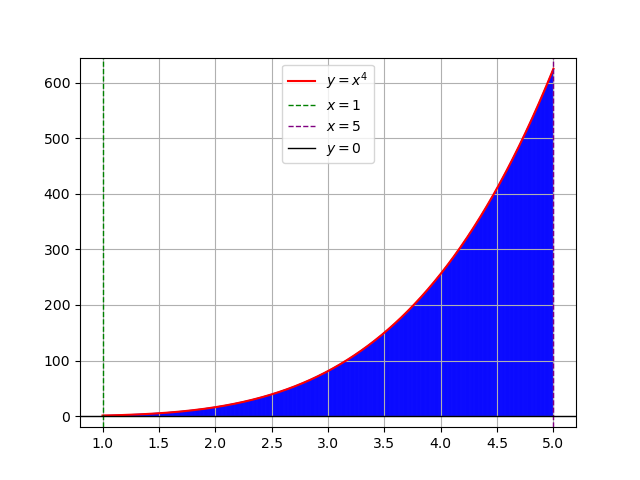
\includegraphics[width=\columnwidth]{figs/plot.png}
    \caption{Plot of the differential equation when $h=0.01$}
    \label{fig:Plot1}
    \end{figure}
\end{document}}
